\begin{title}[\Large]
  Параграф 1.2
\end{title}

\begin{title}[\Large]
  Эквивалентные параметризации кривой. Определение и свойства натурального
  параметра
\end{title}

\begin{define}[диффеоморфизма]
  Диффеоморфизмом называется взаимооднозначаное и гладкое отображение при
  котором обратное отображение тоже гладкое.

  Биективное отображение гладкое в обе стороны.
\end{define}

\begin{define}[эквивалентных кривых]
  $\varphi_1 : [a,b] \to R^3$

  $\varphi_2 : [\alpha, \beta] \to R^3$

  называются эквивалентными если существует диффeoморфизм то есть
  $\exists \varphi : [a,b] \to [\alpha, \beta] ~~~ \vec \varphi_2
  (\vec \varphi(t)) = \vec \varphi_1(t)$

  Все кривые разбиваются на классы эквивалентных кривых
\end{define}

\begin{block}[Длина дуги кривой]
  $\vec \varphi = \vec \varphi(t)$ регулярная кривая, тогда длина дуги кривой
  $$
  s = \int_{t_0}^{t_1} | \vec \varphi'(t)| dt
  $$
  $$
  \vec \varphi'(t) =
  \left\{
  \begin{array}{c}
    x = x(t) \\
    y = y(t) \\
    z = z(t)
  \end{array}
  \right. ~~~~
  s = \int_{t_0}^{t_1} \sqrt{ x'^2(t) + y'^2(t) + z'^2(t)}
  $$
\end{block}

\begin{define}[натуральной параметризации кривой]
  Параметризация при которой каждой точке кривой сопаставляется длина
  кривой от точки до некоторой фиксированной точки называется натуральной или
  естественной параметризацией.
\end{define}

\begin{block}[Свойства]
  1) Натуральная параметризация эквивалентна исходной параметризации.

  \begin{proof}
    $\vec \varphi = \vec \varphi(t)$ кривая

    $s = s(t)$ натуральная параметризация
    $$
    \int_{t_0}^{t_1} |\vec \varphi'(t)| dt ~~~
    \frac{ds}{dt} = |\vec \varphi'(t)| > 0
    $$
    $\Rightarrow ~ s = s(t) ~ \nearrow ~ \Rightarrow ~ s = s(t)$ биективна
    $\Rightarrow$ диффеоморфна
  \end{proof}

  2) $\left| \frac{d \vec \varphi}{ds} \right| = 1$ то есть для любой точки
  натурально параметризованной кривой касательный вектор имеет длину $1$

  \begin{proof}
    $$
    \vec \varphi(s) = \vec \varphi (t(s))
    $$
    $$
    S = \int_{t_0}^{t_1} |\vec \varphi'(t)| dt ~ \Rightarrow ~ \frac{ds}{dt} =
    |\vec \varphi'(t)|
    $$
    $$
    \frac{d\vec \varphi}{ds} = \frac{d \vec \varphi}{dt} \frac{dt}{ds} =
    \vec \varphi' \cdot \frac{1}{|\vec \varphi'|} ~ \Rightarrow ~ \vec \varphi'
    ~ \text{вектор длины 1}
    $$
  \end{proof}

  \begin{block}[Лемма]
    Если $|\vec \varphi(t)| = \const$ тогда $\vec \varphi'(t) \perp
    \vec \varphi(t)$
  \end{block}

  \begin{proof}
    $$
    (\vec \varphi, \vec \varphi) = |\vec \varphi|^2 = \const
    $$
    $$
    \frac{d(\vec \varphi, \vec \varphi)}{dt} = (\vec \varphi', \vec \varphi) +
    (\vec \varphi, \vec \varphi') = 2(\vec \varphi', \vec \varphi) = 0 ~
    \Rightarrow ~ \vec \varphi' \perp \vec \varphi
    $$
  \end{proof}

  3)
  $$
  \frac{d^2 \vec \varphi}{ds^2} \perp \frac{d\vec \varphi}{ds}
  $$
  \begin{proof}
    Так как $\left| \frac{d\vec \varphi}{ds} \right| = 1 = const$ тогда
    по лемме $\frac{d^2 \vec \varphi}{ds^2} \perp \frac{d\vec \varphi}{ds}$
  \end{proof}
\end{block}

\begin{title}[\Large]
  Кривизна и кручение кривой: определение, геометрический смысл, свойства
\end{title}

\begin{define}[кривизны кривой]
  $$
  k =
  \left|
    \frac{d^2 \vec \varphi}{d s^2}
  \right| ~~~
  \text{называется кривизной кривой}
  $$
  $$
    \frac{d^2 \vec \varphi}{d s^2} ~~~ \text{вектор кривизны}
  $$
  Величина, обратная кривизне кривой $r = \frac{1}{k}$ называется радиусом
  кривизны который совпадает с радиусом соприкасающейся окружности в данной
  точке кривой. Центр этой окружности называется центром кривизны. Если кривизна
  кривой равна нулю, то соприкасающаяся окружность вырождается в прямую.

  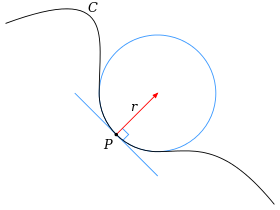
\includegraphics[width = 4.5cm]{Osculating_circle}
\end{define}

\begin{theorem}
  Кривизна кривой $k = 0$ $\Leftrightarrow$ ее образ является прямой.
\end{theorem}

\begin{proof}
  $\Rightarrow ~ k = 0$ тогда
  $$
  \left| \frac{d^2 \vec \varphi}{ds^2} \right| = 0 ~ \Rightarrow ~
  \frac{d^2 \vec \varphi}{ds^2} = \vec 0 ~ \Rightarrow ~
  \frac{d\vec \varphi}{d s} = \vec a = const ~ \Rightarrow ~
  \vec \varphi = \vec a s + \vec b
  $$
  $\Leftarrow ~ k = 0$ тогда
  $$
  \vec \varphi = \vec a s + \vec b  ~ \Rightarrow ~
  \frac{d^2 \vec \varphi}{ds^2} = \vec 0 ~ \Rightarrow ~ k = 0
  $$
\end{proof}

\begin{block}[Лемма]
  $$
  \frac{d\vec b}{ds} ~ || ~ \vec n
  $$
\end{block}

\begin{proof}
  $\vec b = \vec b(s)$ докажем что $\frac{d \vec b}{ds} \perp \vec t, \vec b$

  $|\vec b| = 1 = \const ~ \Rightarrow ~ \frac{d\vec b}{ds} \perp \vec b$
  (по лемме)
  $$
  \vec b = [\vec t, \vec n] ~ \Rightarrow ~ \frac{d\vec b}{ds} =
  \cancelto{\vec 0}{\left[\frac{d \vec t}{ds}, \vec n\right]} +
  \left[\vec t, \frac{d\vec n}{ds}\right] =
  \left[\vec t, \frac{d\vec n}{ds}\right] ~ \Rightarrow ~ \frac{d\vec b}{ds}
  \perp \vec t ~ \Rightarrow ~  \frac{d\vec b}{ds} ~ || ~ \vec n
  $$
\end{proof}

\begin{define}[кручения кривой]
  $\frac{d\vec b}{ds} = -\kappa \vec n$ где $\kappa$ называется кручениче кривой
  в точке.
\end{define}

\begin{theorem}
  Кручение кривой равно $\kappa = 0$ $\Leftrightarrow$ образ кривой лежит в
  плоскости
\end{theorem}

\begin{proof}
  $\Rightarrow$ $\kappa = 0$ тогда
  $$
  \frac{d\vec b}{ds} = \vec 0 ~ \Rightarrow ~ \vec b = (\alpha, \beta, \gamma)
  ~~~ \alpha, \beta, \gamma \in R
  $$
  $$
  \frac{d(\vec \varphi, \vec b)}{ds} = \left(\frac{d \vec \varphi}{ds},
  \vec b \right) + \left( \vec \varphi, \frac{d\vec b}{ds} \right) = 0 ~
  \Rightarrow ~ (\vec \varphi, \vec b) = \const ~ \Rightarrow
  $$
  кривая $\vec \varphi = \vec \varphi (s)$ лежит в плоскости $\alpha x +
  \beta y + \gamma z = D$

  $\Leftarrow$ Пусть кривая лежит в некоторой плоскости тогда
  $\vec b = \const ~ \Rightarrow ~ \frac{d \vec b}{ds} = \vec 0 ~ \Rightarrow ~
  \kappa = 0$
\end{proof}

\begin{block}[Геометрический смысл кривизны и кручения кривой]
  1) Для плоской кривой $k = \left|\frac{d \vec t}{ds}\right|$ равна
  скорости вращения касательного вектора.

  2) $\kappa = \left|\frac{d\vec b}{ds}\right|$ равна скорости вращения
  соприкасающейся плоскости относительно касательной прямой.
\end{block}

\begin{theorem}
  $\forall$ гладких функций $k = k(s) > 0$ и $\kappa = \kappa(s)$ $\exists!$
  с точностью до пложения в пространстве кривая
  $\vec \varphi = \vec \varphi(s)$ кривизна которой и кручение равны то есть
  кривизна и кручение определяют кривую однозначно.
\end{theorem}